\documentclass[a4paper,10pt]{article}
\usepackage[utf8]{inputenc}
\usepackage[margin=0.8in]{geometry}
\usepackage{graphicx}
\usepackage[english]{isodate}
\usepackage[document]{ragged2e}
\graphicspath{ {./img/} }
\usepackage{amsmath}
\usepackage{makecell}
\usepackage{longtable}
\usepackage{hyperref}
\usepackage{url}
\usepackage{textcomp}

\title{DSGA1011 Homework 1: Bag of N-grams Classification}
\author{Rong Feng - rf1316}
\date{\printdayoff\today}

\begin{document}

%\maketitle
Rong Feng, rf1316, Oct 2018, DS-GA1011 HW1: Bag of N-grams Classification \\ 
Public GitHub: \footnote{\url{https://github.com/rmfeng/ds1011_public/tree/master/hw1}}

\section{Summary}
\par 
\justify
As specified in the assignment description, this exercise uses bag-of-ngrams and a fully connected linear layer to classify positive and negative IMDB reviews. The final validation accuracy achieved after hyperparameter optimization was 90.9\% and the final test accuracy was 90.1\%. 

\par
\justify
Following the assignment recommendation, the training set size was set to 20000 and validation to 5000. The test set of 25000 was only used at the end to provide the test accuracy and not touched or optimized over in any other way. The final model hyperparameters are indicated in Table \ref{tbl:finalhparams}. The model took 25mins to run on a single GPU and early stopped after 24 epochs

\begin{table}[!htbp]
\begin{tabular}{| l | l | l |}
\hline
Hyperparameter   & Description                                & Final Model    \\
\hline
LR               & Learning Rate on used Optimizer            & 0.001          \\
LR\_DECAY\_RATE  & Gamma decay rate per epoch                 & 0.95           \\
NEPOCH           & Number of Total Epochs                     & 50             \\
VOC\_SIZE        & Vocab Size                                 & 2 million      \\
EMBEDDING\_DIM   & Embedding Vector Dimension                 & 100            \\
NGRAM\_N         & Size of largest ngram                      & 4              \\
NGRAM\_MODE      & mode of tokenizer (spacy, naive)           & spacy          \\
REMOVE\_STOP     & Whether to remove stop words               & False          \\
REMOVE\_PUNC     & Whether to remove punctuation              & True           \\
EARLY\_STOP      & Whether to consider early stop             & True           \\
ES\_LOOKBACK     & \# of steps to look back for improvement   & 16             \\
ES\_MIN\_IMPROVE & Minimum improvement required for ES        & 0.01           \\
OPTIMIZER        & PyTorch Optimizer Used                     & Adam           \\
\hline
\end{tabular}
\caption{Final Hyperparameters}\label{tbl:finalhparams}
\end{table}

\par
\justify
Three correct predictions in the validation set were: \\{/train/pos/2871\_10.txt}, {/train/neg/10085\_3.txt}, {/train/pos/10366\_10.txt}

\par
\justify
Three incorrect predictions in the validation set were: \\{/train/neg/2304\_1.txt}, {/train/neg/3772\_2.txt}, {/train/neg/7120\_4.txt} (Due to paper space constraints the full texts are redacted here, please look them up from the assignment provided data source)

\section{Architecture}
As specified in the assignment, the model architecture is simply a ngram embedding lookup layer, followed by sum function to encode the bag-of-ngrams, and finally a fully-connected linear layer that outputs the logit of the predicted classes. The used loss was binary cross entropy loss. The formulas and architecture diagrams are redacted here to save room, however are easily accessible online.

\section{Data Preparation}
\par
\justify
Using the github code base for the assignment in 2017 as a starting point, functionality was added to perform the required data preparation \cite{repo2017}. These functionalities include: Tokenization, ngram extraction, building and indexing the vocabulary, and finally loading the data into the PyTorch DataLoader pipeline. Each of these functionalities and their associated hyperparameters are described below:

\par
\justify
\textbf{Tokenization:} To convert the raw text of the reviews to lists of tokens two methods were employed: "naive" and "spacy" \cite{repospacy} methods. For the naive method, the sentences were tokenized by splitting them with the space delimiter. For the spacy method, the smart-tokenization implementation of spacy was called on the input sentence. For example under spacy, "don't" is tokenized into "do" and "n't", extracting the meaning out of the english abbreviation. In both methods both stop words and punctuation are moved if specified by their respective hyperparameters.

\par
\justify
\textbf{Ngram Extraction:} From the list of tokens, iterate through them to extract all ngrams of size equal or less than the specified hyperparameter. 

\par
\justify
\textbf{Building Vocabulary:} Using the python Counter object, take the top n most frequently occurring ngrams and form our vocabulary of ngrams, where n is determined by the VOC\_SIZE hyperparameter. For each input review, its ngrams are then mapped to the index of that ngram in the vocabulary. All encountered ngrams that do not belong to the vocabulary are mapped to a special \textlangle{}unk\textrangle{} placeholder. Further, a special \textlangle{}pad\textrangle{} placeholder is added at index 0 in the vocabulary used for input padding.

\par
\justify
\textbf{Converting to PyTorch DataLoader:} Finally, a collate function was implemented in PyTorch's required format. It takes the ngram indexes of the inputs and converts a batch of inputs into a PyTorch Tensor representation. The input data is also wrapped by the DataLoader to take advantage of various convenience implementations in the pytorch DataLoader such as shuffling and batching.

\section{Establishing Baseline}
Starting with heuristically selected hyperparamters, the "heuristic model" uses lab examples and other implementations as the heuristic. Basic ablation analysis was then run over single or sets of hyperparameters to arrive at our "baseline model" with the following hyperparameters in Table \ref{tbl:hyperparams}.  Further hyperparameters optimization is described in Section \ref{furthertuning} to arrive at the final model.

\begin{table}[!htbp]
\begin{tabular}{| l | l | l | l |}
\hline
Hyperparameter   & Description                                &  Heuristic & Baseline  \\
\hline
LR               & Learning Rate on used Optimizer            & 0.01             & 0.01           \\
LR\_DECAY\_RATE  & Gamma decay rate per epoch                 & 1                & 0.95           \\
NEPOCH           & Number of Total Epochs                     & 10               & 10             \\
VOC\_SIZE        & Vocab Size                                 & 10k              & 100k           \\
EMBEDDING\_DIM   & Embedding Vector Dimension                 & 100              & 50             \\
NGRAM\_N         & Size of largest ngram                      & 2                & 4              \\
NGRAM\_MODE      & mode of tokenizer (spacy, naive)           & naive            & spacy          \\
REMOVE\_STOP     & Whether to remove stop words               & True             & False          \\
REMOVE\_PUNC     & Whether to remove punctuation              & True             & True           \\
EARLY\_STOP      & Whether to consider early stop             & True             & True           \\
ES\_LOOKBACK     & \# of steps to look back for improvement & 2                & 8              \\
ES\_MIN\_IMPROVE & Minimum improvement required for ES        & 0.01             & 0.01           \\
OPTIMIZER        & PyTorch Optimizer Used                     & Adam             & Adam           \\
\hline
\end{tabular}
\caption{Baseline Hyperparameters}\label{tbl:hyperparams}
\end{table}

\par
\justify
The heuristic model achieved a validation accuracy of 87.5\% after 2.0 epochs and exits due to the early stop condition being met. The baseline model achieved a validation accuracy of 88.9\% after 4.0 epochs and exits due to the early stop condition being met. The training and validation curves for the baseline model are shown in Figure \ref{fig:trainvalcurves}. To arrive at the baseline model from the heuristic model, some simple ablation analysis are performed as described below.

\begin{figure}[h]
    \centering
    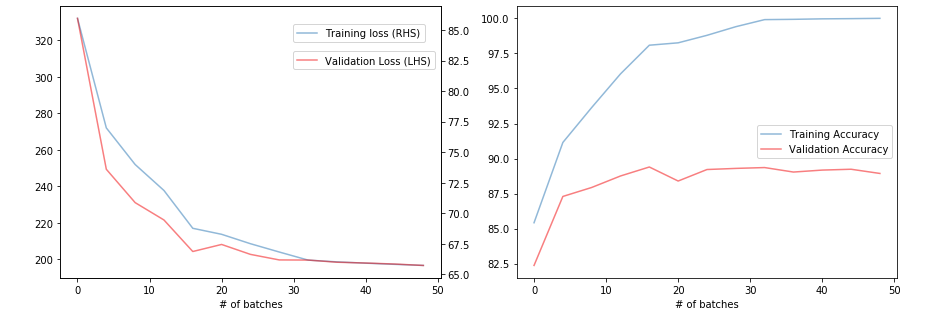
\includegraphics[scale=0.4]{trainvalcurves}
    \caption{Baseline Training and Validation Curves}
    \label{fig:trainvalcurves}
\end{figure}

\par
\justify
\textbf{Learning Rate:} The learning rate parameter was for the baseline was kept at 0.01 after running the baseline model for 1 epoch by only adjusting the learning rate. Similar to the methodology performed in \cite{learningrate} the best performance was found to be at 0.01. Figure \ref{fig:lrexplore}


\begin{figure}[h]
    \centering
    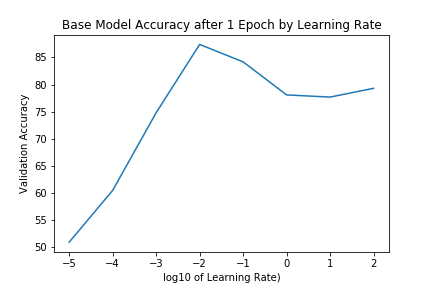
\includegraphics[scale=0.3]{lr_explore}
    \caption{Baseline ablation by learning rate}
    \label{fig:lrexplore}
\end{figure}


\par
\justify
\textbf{Embedding Dimension:} The embedding dimension ablation study was performed in conjunction with adjusting vocabulary sizes in a small range between 20k and 120k. It was found that although there is variability caused by the vocabulary sizes, increasing the embedding dimension would on average decrease the validation accuracy. As a result embedding dimension was reduced to 50 from the heuristic value of 100.

\begin{figure}[h]
    \centering
    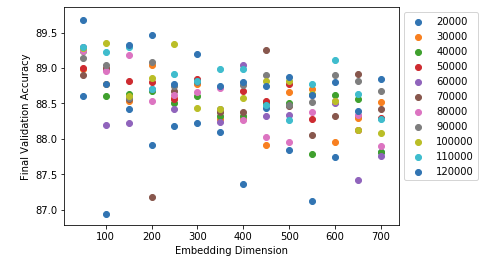
\includegraphics[scale=0.4]{embedding}
    \caption{Declining Performance of Embedding Size}
    \label{fig:embedding}
\end{figure}


\par
\justify
\textbf{Tokenization Scheme Parameters:} First, to select either spacy or naive tokenization, the accuracies achieved using the two tokenization styles for different vocabulary sizes and ngram sizes was computed. In Figure \ref{fig:spacynaive}, note that across vocabulary sizes, spacy generally out performs their naive counter parts. As a result spacy was chosen as the tokenization method. Subsequently, all of the 4 combinations of REMOVE\_STOP, REMOVE\_PUNC were tried with all other hyperparameters under the baseline conditions, the results are in Figure \ref{fig:spacyoptions}. The best result was used as baseline: \{spacy, REMOVE\_STOP=False, REMOVE\_PUNC=True\}

\begin{figure}[h]
    \centering
    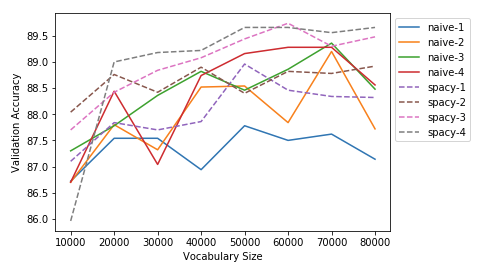
\includegraphics[scale=0.4]{spacynaive}
    \caption{Spacy vs. Naive Tokenization}
    \label{fig:spacynaive}
\end{figure}

\begin{figure}[h]
    \centering
    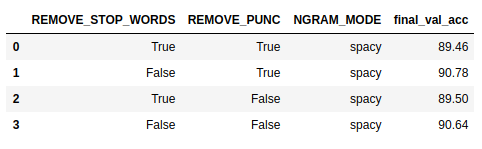
\includegraphics[scale=0.4]{spacyoptions}
    \caption{Spacy Punctuation and Stop Words}
    \label{fig:spacyoptions}
\end{figure}

\par
\justify
\textbf{Ngram Size:} Using the same analysis as used when considering the tokenization scheme, notice that performance is improved as ngram size increases. Figure \ref{fig:spacynaive}. For the baseline, NGRAM\_N was increased the maximum specified in the assignment of 4.

\par
\justify
\textbf{Vocabulary Size:} Even with very large vocabulary sizes, the set of all 4grams covered by that vocabulary remains low. At a vocab size of 1 million, only 46\% of the set of all ngrams are covered by that vocabulary so there is even more room to increase the vocabulary size. As observed in Figure \ref{fig:vocabsize}, increasing the vocab size does improve performance. However, the run time is significantly increased by the vocabulary size and thus to keep the baseline model fast for ablation analysis, a baseline size of 100k was selected. Larger vocabulary sizes will be explored in Section \ref{furthertuning} below.


\begin{figure}[h]
    \centering
    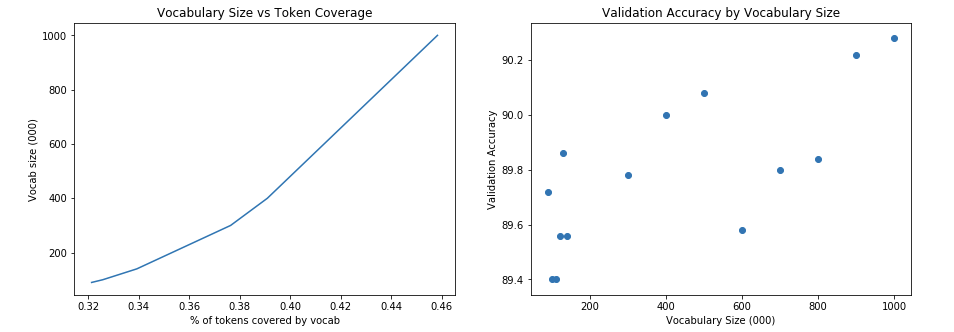
\includegraphics[scale=0.3]{vocabsize}
    \caption{Exploring Vocabulary Size}
    \label{fig:vocabsize}
\end{figure}

\par
\justify
\textbf{Optimizer:} Finally, SGD, Adadelta, RMSprop and Adam were trialed as possible optimizers, with Adam achieving the top validation accuracy after 2 epochs. As a result, Adam remained the baseline optimizer. The training curves are redacted here due to space, but can be found in Hyperparam Opt.ipynb of the GitHub submission.

\section{Further Hyperparameter Tuning}\label{furthertuning}
To further optimize for the final few points of performance, a slower specification was crafted with a much larger vocabulary size. The slow model vocabulary size was increased to 2 million, the learning rate was decreased by a factor of 10, and decayed at a factor of 0.95 each epoch. The early stop condition was increased to a lookback period of 16 steps (64 batches) and max epoch increased to 50. The training curves are depicted below in Figure \ref{fig:finalcurve}. The reported test accuracy is from this model.

\begin{figure}[h]
    \centering
    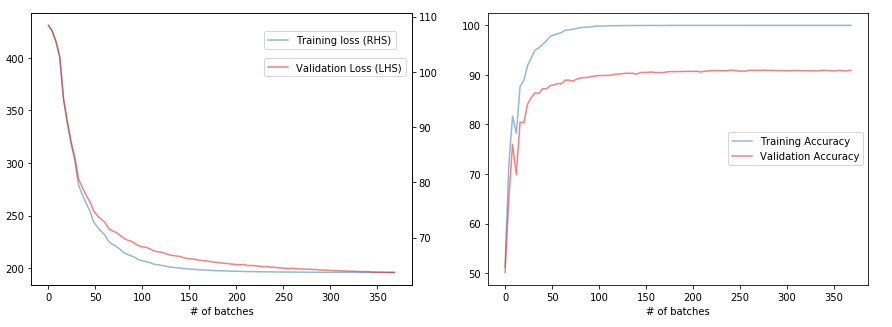
\includegraphics[scale=0.4]{finalcurve}
    \caption{Final Training Curve}
    \label{fig:finalcurve}
\end{figure}

\medskip

\bibliographystyle{unsrt}%Used BibTeX style is unsrt
\bibliography{refs}

\end{document}
